\begin{tehtavasivu}

% tässä ei käytetä konsistenssin vuoksi euromerkkiä \euro (textmode), vaan sanallista ilmaisua ''euro''

% FIXME: Tee vielä toinen tehtävä perusarvosta ``Kirjan myyntihinta'' -tehtävän lisäksi

% FIXME: laaja tehtävä ansio- ja pääomatulojen verotuksesta
\subsubsection*{Opi perusteet}

\begin{tehtava}
Täydennä taulukko.
\begin{tabular}{|c|c|c|c|}
\hline 
desimaaliluku & (supistettu) murtoluku & \% & \permil \\ 
\hline 
$0,1$ & & & \\ 
\hline 
 & $-\frac{4}{5}$ & & \\ 
\hline 
 & & $99,9$ & \\ 
\hline 
 & & & $0,42$ \\ 
\hline 
 & & $125$ & \\ 
 \hline
$-7,5$  & & & \\
  \hline
\end{tabular}
\begin{vastaus}
\begin{tabular}{|c|c|c|c|}
\hline 
desimaaliluku & (supistettu) murtoluku & \% & \permil \\ 
\hline 
$0,1$ & $\frac{1}{10}$&$10$ &$100$ \\ 
\hline 
$0,8$ & $-\frac{4}{5}$ & $80$ & $800$\\ 
\hline 
$0,999$ & $\frac{999}{1\,000}$& $99,9$ & $999$\\ 
\hline 
$0,00042$ &$\frac{21}{50\,000}$ & $0,042$& $0,42$ \\ 
\hline 
$1,25$ &$\frac{5}{4}$ & $125$ & $1\,250$\\ 
 \hline
$-7,5$ & $-\frac{15}{2}$& $-750$&$-7\,500$ \\
  \hline
\end{tabular}
\end{vastaus}
\end{tehtava}
\begin{tabular}{|c|c|c|c|}
\hline 
perusarvo & $\pm p$\,\% & prosenttikerroin & lauseke \\ 
\hline 
$a$ & $+10$\,\% & $1,10$ & $1,10a$ \\ 
\hline 
$b$ & $+2,4$\,\% & & \\ 
\hline 
$5\,000$\,€ & & $99,9$ & \\ 
\hline 
 & & & $0,42x$ \\ 
\hline 
 $3$\,m& & 125 & \\ 
 \hline
  & & &$0,003\cdot(-7,5)$ \\
  \hline
\end{tabular}
\begin{tehtava}
Täydennä taulukko.
\begin{tabular}{|c|c|c|c|}
\hline 
perusarvo & $\pm p$\,\% & prosenttikerroin & lauseke \\ 
\hline 
$a$ & $+10$\,\% & $1,10$ & $1,10a$ \\ 
\hline 
$b$ & $+2,4$\,\% & & \\ 
\hline 
$5\,000$\,€ & & $99,9$ & \\ 
\hline 
 & & & $0,42x$ \\ 
\hline 
 $3$\,m& & 125 & \\ 
 \hline
  & & &$0,003\cdot(-7,5)$ \\
  \hline
\end{tabular}

\begin{vastaus}

\end{vastaus}

\end{tehtava}




\begin{tehtava}
    Laske
    \alakohdat{
	  § $4,5\,\%$ luvusta $1\,500$
	  § $4,5\,\%$ luvusta $b$
	  § $15,3\,\%$ luvusta $b$
	  § $152\,\%$ luvusta $b$
	  § $3\,550\,\%$ luvusta $b$.
    }
    \begin{vastaus}
	  \alakohdat{
		§ $67,5$
		§ $0,045b$
		§ $0,153b$
		§ $1,52b$
		§ $35,5b$
	  }
    \end{vastaus}
\end{tehtava}

\begin{tehtava}
    Kuinka monta prosenttia
    \alakohdat{
	  § $15$ on luvusta $75$
	  § $120$ on luvusta $80$
	  § $400$ on luvusta $3,5$
	  § luku $50$ on lukua $170$ pienempi
	  § luku $170$ on lukua $50$ suurempi
	  § $400$ on lukua $3,5$ suurempi?
    }
    \begin{vastaus}
	  \alakohdat{
		§ $20$\,\%
		§ $150$\,\%
		§ $11\,428,6$\,\%
		§ $70,6$\,\%
		§ $240$\,\%
		§ $11\,328,6$\,\%
	  }
    \end{vastaus}
\end{tehtava}


\begin{tehtava}
    Laukun normaalihinta on $225$ euroa, ja se on $25$ prosentin alennuksessa. Mikä on alennettu hinta?
    \begin{vastaus}
        $168,75$ euroa
    \end{vastaus}
\end{tehtava}

\begin{tehtava}
    Jaakon kuukausipalkka on $1\,623,52$ euroa. Hän saa $1,3\,\%$ palkankorotuksen. Mikä on Jaakon kuukausipalkka korotuksen jälkeen?
    \begin{vastaus}
        $1644,63$ euroa
    \end{vastaus}
\end{tehtava}

\begin{tehtava}
    Kirjan myyntihinta, joka sisältää arvonlisäveron, on $9\,\%$ suurempi kuin kirjan veroton hinta. Laske kirjan veroton hinta, kun myyntihinta on $27$ euroa.
    \begin{vastaus}
        Kirjan veroton hinta on $24,77$ euroa.
    \end{vastaus}
\end{tehtava}

\begin{tehtava}
	Avoin kierros laserhippaa (laser tag) maksaa yhdeltä pelaajalta $9$ euroa. Pelialueen voi kuitenkin varata seurueelle hintaan $260$ euroa. Mette on menossa pelaamaan viiden kaverinsa kanssa. 
	\alakohdat{
		§ Kuinka monta prosenttia kalliimpaa on varata joukolle yksityispeli kuin liput avoimeen peliin?
		§ Kuinka suuri seurueen on vähintään oltava, jotta yksityispeli tulisi halvemmaksi?
	}
	\begin{vastaus}
		\alakohdat{
			§ $381\,\%$
			§ $29$
		}
	\end{vastaus}

\end{tehtava}

\begin{tehtava}
    Samulin pituus on $165$\,cm ja Joonaksen $173$\,cm.
    \alakohdat{
        § Kuinka monta prosenttia Samulin pituus on Joonaksen pituudesta?
        § Kuinka monta prosenttia Joonaksen pituus on Samulin pituudesta?
        § Kuinka monta prosenttia Samuli on lyhyempi kuin Joonas?
        § Kuinka monta prosenttia Joonas on pidempi kuin Samuli?
    }
    \begin{vastaus}
        \alakohdat{
            § $95,4\,\%$
            § $104,8\,\%$
            § $4,62\,\%$
            § $4,85\,\%$
        }
    \end{vastaus}
\end{tehtava}

\begin{tehtava}
    Jalkapalloilija Georgios Samaras teki ensimmäisellä kaudellaan Skotlannin valioliigassa (2007--2008) $5$ maalia Celtic F.\,C.:n paidassa. Seuraavalla kaudella Samaras teki Celticille liigassa $15$ maalia. Kuinka monta prosenttia Samaraksen maalimäärä nousi?
    \begin{vastaus}
        $200\,\%$
    \end{vastaus}
\end{tehtava}

\subsubsection*{Hallitse kokonaisuus}

\begin{tehtava}
    Sokerijuurikkaassa on $18\,\%$ sokeria. Kuinka paljon sokerijuurikkaita tarvitaan valmistettaessa $8$ tonnia sokeriliuosta, jonka sokeripitoisuus on $4,5\,\%$?
    \begin{vastaus}
        $2$ tonnia
    \end{vastaus}
\end{tehtava}

\begin{tehtava}
    Piraattipuolueen kannatus oli vuoden 2011 eduskuntavaaleissa $0,5\,\%$ ja vuoden 2014 europarlamenttivaaleissa $0,7\,\%$. Kuinka monta prosenttiyksikköä kannatus nousi? Kuinka monta prosenttia kannatus nousi?
    \begin{vastaus}
        Kannatus nousi $0,2$ prosenttiyksikköä ja toisaalta $40$ prosenttia. (Tiedotusvälineissä kannatusmuutokset ilmoitetaan yleensä prosenttiyksiköissä.)
    \end{vastaus}
\end{tehtava}

\begin{tehtava}
    Askartelukaupassa on alennusviikot ja kaikki tavarat myydään $60\,\%$:n alennuksella. Viimeisenä päivänä kaikista hinnoista annetaan vielä lisäalennus, joka lasketaan aiemmin alennetusta hinnasta. Minkä suuruinen lisäalennus tulee antaa, jos lopullisen kokonaisalennuksen halutaan olevan $80\,\%$?
    \begin{vastaus}
        $50\,\%$
    \end{vastaus}
\end{tehtava}

\begin{tehtava}
    Oppikirjamaraton-tiimi kävi lounastamassa. Osoita oheisen kuitin tiedoilla vääräksi yleinen virhekäsitys, että $13\,\%$ suuruisen arvonlisäveron osuus olisi $13\,\%$ lopullisesta myyntihinnasta.
    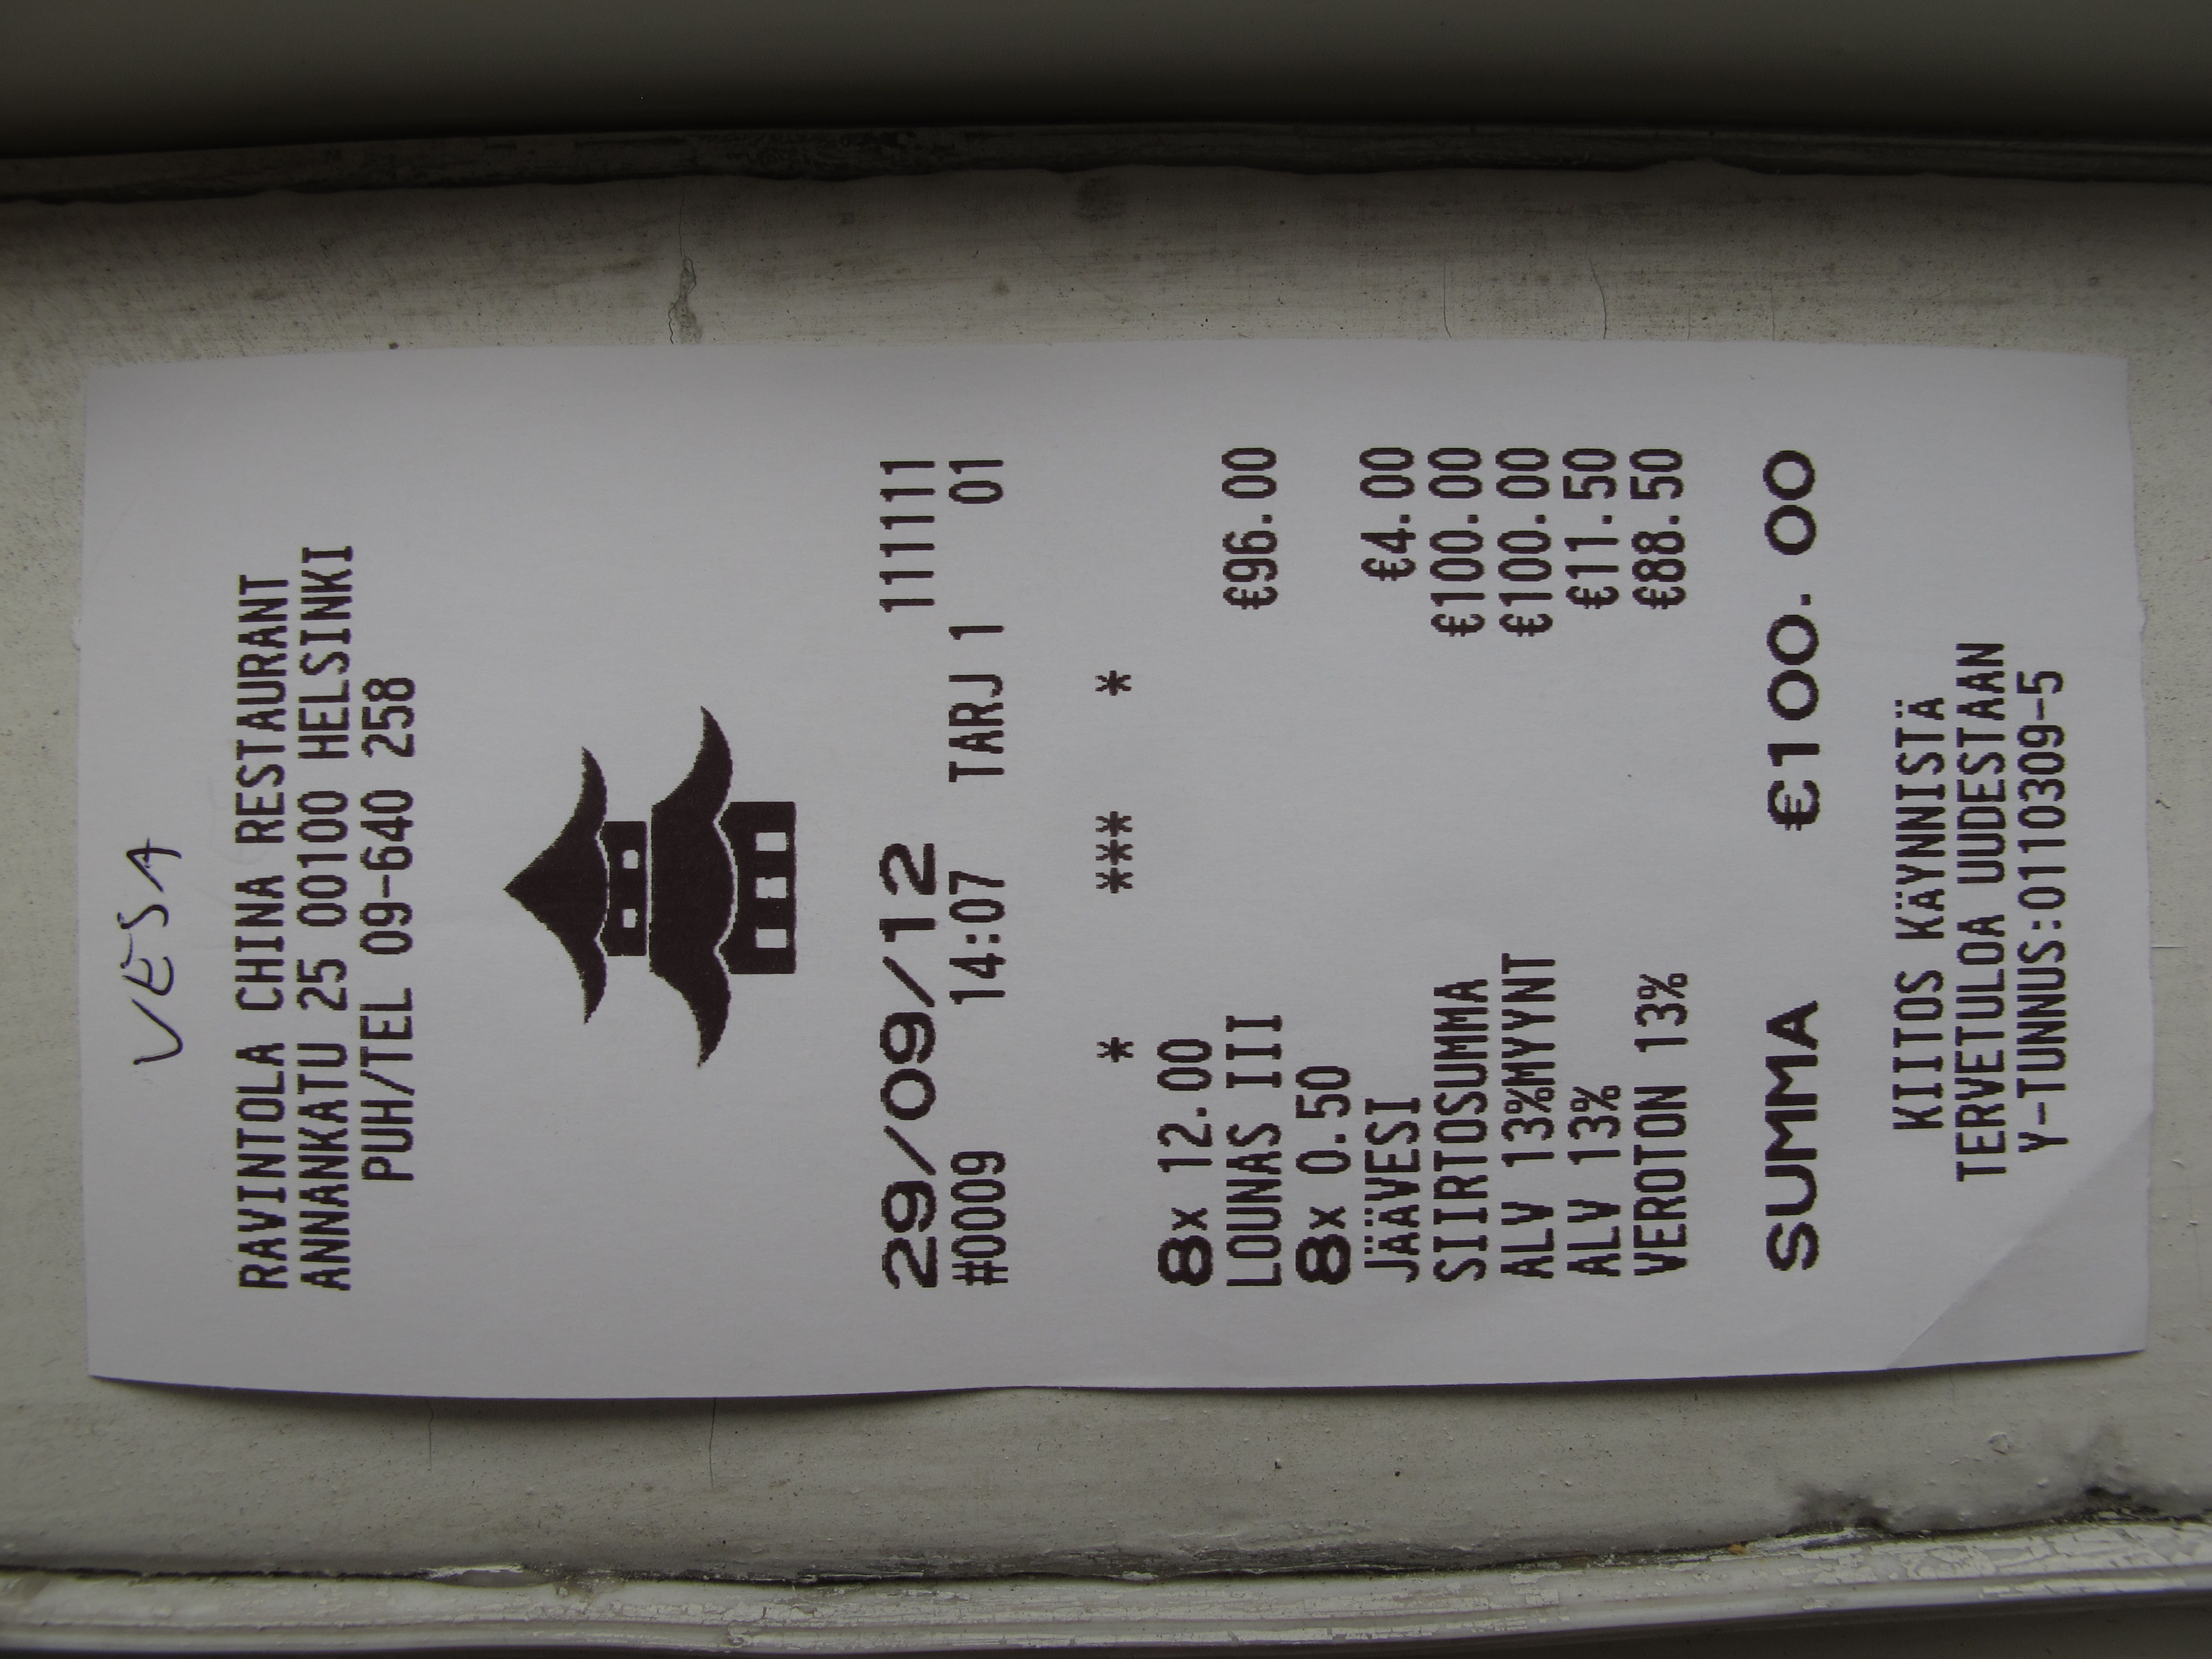
\includegraphics[width=80mm, angle=270]{pictures/alv-kuitti}
    \begin{vastaus}
         $13\,\%$ sadasta eurosta on $13$ euroa, ei $11,50$ euroa, niin kuin kuitissa todetaan. Arvonlisävero lasketaan suhteessa verottomaan hintaan, ei lopulliseen myyntihintaan.
    \end{vastaus}
\end{tehtava}

\begin{tehtava}
    Hedelmissä on vettä aluksi $60\,\%$ niiden painosta. Kuinka monta prosenttia vedestä on haihdutettava, jotta hedelmissä tämän jälkeen olisi vain $20\,\%$ vettä?
    \begin{vastaus}
        $\approx83,3\,\%$
    \end{vastaus}
\end{tehtava}

\begin{tehtava}
    (YO 2000K/4) Tuoreissa omenissa on vettä $80\,\%$ ja sokeria $4\,\%$. Kuinka monta prosenttia sokeria on samoissa omenissa, kun ne on kuivattu siten, että kosteusprosentti on $20$?
    \begin{vastaus}
        $16\,\%$
    \end{vastaus}
\end{tehtava}

\begin{tehtava}
    Erään pankin myöntämä opintolaina kasvaa korkoa $2\,\%$ vuodessa. Kuinka monta prosenttia laina on kasvanut korkoa alkuperäiseen verrattuna kymmenen vuoden kuluttua?
    \begin{vastaus}
        $22\,\%$.
    \end{vastaus}
\end{tehtava}

\begin{tehtava}
    Vuonna 2012 yleinen arvonlisäveroprosentti Suomessa oli $23\,\%$ tuotteen verottomasta hinnasta. Tuotteen hinta koostuu sen verottomasta hinnasta ja tuotteesta maksettavasta arvonlisäverosta. Kuinka monta prosenttia arvonlisävero on tuotteen myyntihinnasta?
    \begin{vastaus}
        $18,7\,\%$
    \end{vastaus}
\end{tehtava}

\begin{tehtava}
    Kun matkalipun hintaa korotettiin $10,0\,\%$, matkustajien määrä väheni $10,0\,\%$. Kuinka monella prosentilla tällöin kasvoivat tai vähenivät liikennöitsijän lipputulot?
    \begin{vastaus}
        Lipputulot vähenivät $1$\,prosentilla.
    \end{vastaus}
\end{tehtava}

\subsubsection*{Lisää tehtäviä}

%Lisännyt Aleksi Sipola 10.11.2013
\begin{tehtava}
    (YO 1991K/5a) Luvun $\sqrt{r^2-a^2}$ likiarvona voidaan käyttää lukua $r-{\frac{1}{2}a^2}/r$. Laske tämän nojalla $\sqrt{3}$ likiarvo sopivia kokonaislukuja r ja a käyttäen. Kuinka monta prosenttia tämä likiarvo poikkeaa tarkasta arvosta?
    \begin{vastaus}
        Likiarvo on $1,75$ ja $\sqrt{3}=1,732...$ Likiarvo poikkeaa noin $1,04\,\%$.
    \end{vastaus}
\end{tehtava}

\begin{tehtava}
    Matin ja Iidan duo saa julkisuutta, ja he alkavat myydä CD-levyään keikkojen yhteydessä $10$ euron kappalehinnalla. Jonkin ajan päästä he päättävät laskea CD-levyn hintaa $20$ prosenttia. Matti alkaa kuitenkin katua päätöstä, ja ehdottaa tämän alennetun hinnan korottamista $20$ prosentilla. Mikä olisi tämän toimenpiteen jälkeen CD:n uusi hinta? Montako prosenttia olisi korotuksen oltava, jotta oikeasti päästäisiin takaisin alkuperäiseen $10$ euron hintaan?
    \begin{vastaus}
        $25\,\%$
    \end{vastaus}
\end{tehtava}


\begin{tehtava}
    (YO 1877/4) Kaupungissa tuli jokaisen talonomistajan suorittaa kaupungin kassaan $5\,\%$ saadusta hyyrymäärästä (vuokrasta, ruotsin sanasta \textit{hyra}). Sittemmin määrättiin, että mainittu prosentti oli oleva 10. Monellako prosentilla talonomistajien täytyi korottaa hyyryjä saadakseen saman puhtaan säästön kuin ennen?
    \begin{vastaus}
        $5,6\,\%$
    \end{vastaus}
\end{tehtava}


\end{tehtavasivu}
